%%%%%%%%%%%%%%%%%%%%%%%%%%%%%%%%%%% CAD Interfaces %%%%%%%%%%%%%%%%%%%%%%%%%%%%%%%%%%%%%%%%%%%%%
\clearpage
\section{CAD Interfaces}

\subsection{The University of Wisconsin Unified Workflow}
The University of Wisconsin Unified Workflow, known as (UW)$^2$ is a mechanism by which 
monte carlo code agnostic metadata can be attached into DAGMC geometry. A DAGMC geometry
file is a MOAB database, which when on disk resides as a HDF5 formatted file. The C++
parts of the Python for Nuclear Engineering (PyNE) toolkit are used as a \textit{Lingua Franca}
to aid in the translation of metadata. Specifically, we use the Material, Tally, Particle 
and Name classes.
\subsection{Materials}
The \texttt{Material} class is the most fundamental class is used in UW$^2$, where we create and store
materials in their in memory (object) form, and also where the I/O methods are for the writing 
of the material object. The material object exists as a standard map of integer nuclide ID numbers
and their appropriate mass fractions, when required we have functions available to call which will
write their MC code specific versions, for example to Fluka or MCNP. 
\subsection{Tallies}
\subsection{\texttt{uwuw\_preproc}}
The general workflow of using UW$^2$ is to make a PyNE material library which contains all the materials
which are used in your problem. The \texttt{uwuw\_preproc} tool is then used to extract the material 
objects from the material library and inserts them into the DAGMC geometry file. This DAGMC geometry
file can now be run in any of the UW$^2$ enabled MC codes, but with the knowledge that the same original
material description is used in each code. 
\subsection{Limitations of UW$^2$}
It should be noted, that using the UW$^2$ workflow inputs the same material description, but the MC 
code may not be capable of describing the material in its original description, for example whilst
Fluka can describe any nuclide arbitrarily by defining its density, atomic and nucleon number it only
contains a limited selection for neutron cross sections below 20 MeV, with only the isotopes of 
hydrogen, helium, lithim, boron, iodine, xenon, caesium, uranium and some of plutonium descibed in
any isoptopic way. This means that physics aside, the ``low energy'' neutron material definitions are
inherently different, but this is order to match the requirements of the physics code and not a limitation 
of the workflow itself. Similarly to Fluka, Geant4 when suitable neutron transport cross sections are not 
available it will choose some defaults using the cross sections of nuclides with similar nucleon numbers
and atomic numbers.

\subsection{FluDAG}
The DAGMC implementation using Fluka is known as FluDAG. It uses the FluGG interface that exists
in FLuka. The function wrappers have distinct simple C style function arguments and store any 
C++ state behind this layer. The FluGG interface was originally written under the assumption
that unambiguous results to any of the geometric query functions can be given, such as 
given a particle location, determine the cell it is bounded by. With DAGMC we need to include some
additional state, stored in the RayHistory class which contains information regarding the last triangle
that was crossed, this state (if used) should be reset when we change direction, cross boundaries, and
when a history ends. There is some complexity regarding the internal program flow of Fluka, Specifically
some of the logic of electrons transport ``sensing steps'' and regarding when particles cross boundaries. 
Especially electrons crossing boundaries, which can logically cross a boundary but end up in the cell in 
which it began. The combination of DAGMC state and the need to know when a particle was taking a sensing step 
means that we needed to access a some of the internal Fluka common blocks which complicates some of the
software library design.

\subsection{DagSolid}
\label{dagsolid}
The DAGMC implementation for the Geant4 interface was originally written by the University of Seoul. 
As part of this contract the \textit{DagSolid} implementation was improved upon, modernised,  and a 
suite of unit tests added. A single instance of a \textit{DagSolid} object performs queries only
on a single DAGMC volume, this fits well with the paradigm of Geant4 geometries being hierachical 
geometry objects where parent-child relationships indicate which volumes are bounded by others. 
The \textit{DagSolid} library therefore meets the expectations of the Geant4 geometry interface, it is
entirely possible therefore to mix DAGMC geometry and Geant4 geometry seamlessly as the DagSolid object
will have parents and children well described by Geant4 geometry hierachy, excellent speedup was observed
when used in this mode.
\subsubsection{DagGeant4}
Also to facililtate a better user experience, a dedecated \textit{DagGeant4}  
executable was written which allows the loading and running of the UW$^2$ workflow, 
reading material objects and tallies from the geometry and instanciates the appropriate Geant4 
\texttt{G4Elements}, \texttt{G4Isotopes} and \texttt{G4Materials} and implments an appropriate 
set of \texttt{G4SensitiveDetector}. The DagGeant4 executable has not been formally benchmarked
as part of this work and should be planned as some future work. 
\subsubsection{Limitations}
As described in \ref{sec:dagsolid} a single DagSolid object represents a single DAGMC volume, and allows
all the needed geometric query functions that Geant4 expects. However, because of the nature of the production
route of DAGMC geometries, i.e. a flat geometry hierarchy where imprinted surface information determines
the next volume a ray crosses given a surface, we have no knowledge of any underlying geometry hierarchy. 
Indeed the typical production route of DAGMC geometry removes all hierarchical information, therefore all 
DagSolid volumes in DagGeant4 exist as children of the highest level ``Mother'' volume. This implies a drastic
performance hit as DagGeant4 performs intersections on all volumes at the current level 
\footnote{Geant4 has a smart voxel builder, which should make this query faster than a linear check of 
each volumes, but it currently unknown if a DagSolid returns enough information for the voxel builder.}
and the accepted hit is the nearest intersection, thus utterly defeating the full acceleration allowed
by the OBB Tree. Instead either the \texttt{G4Navigator} needs to made stateful, keeping track of last surface
crossed and therefore making use of the imprint information, or perhaps use \textit{GenerateHierarchy} 
to allow the use of Geant4 parent-child links.
\subsection{HZETran}

\clearpage
\subsection{Benchmarks}
\subsubsection{ATIC}
\clearpage
\begin{figure}[ht!]
 \begin{centering}
 \centering
 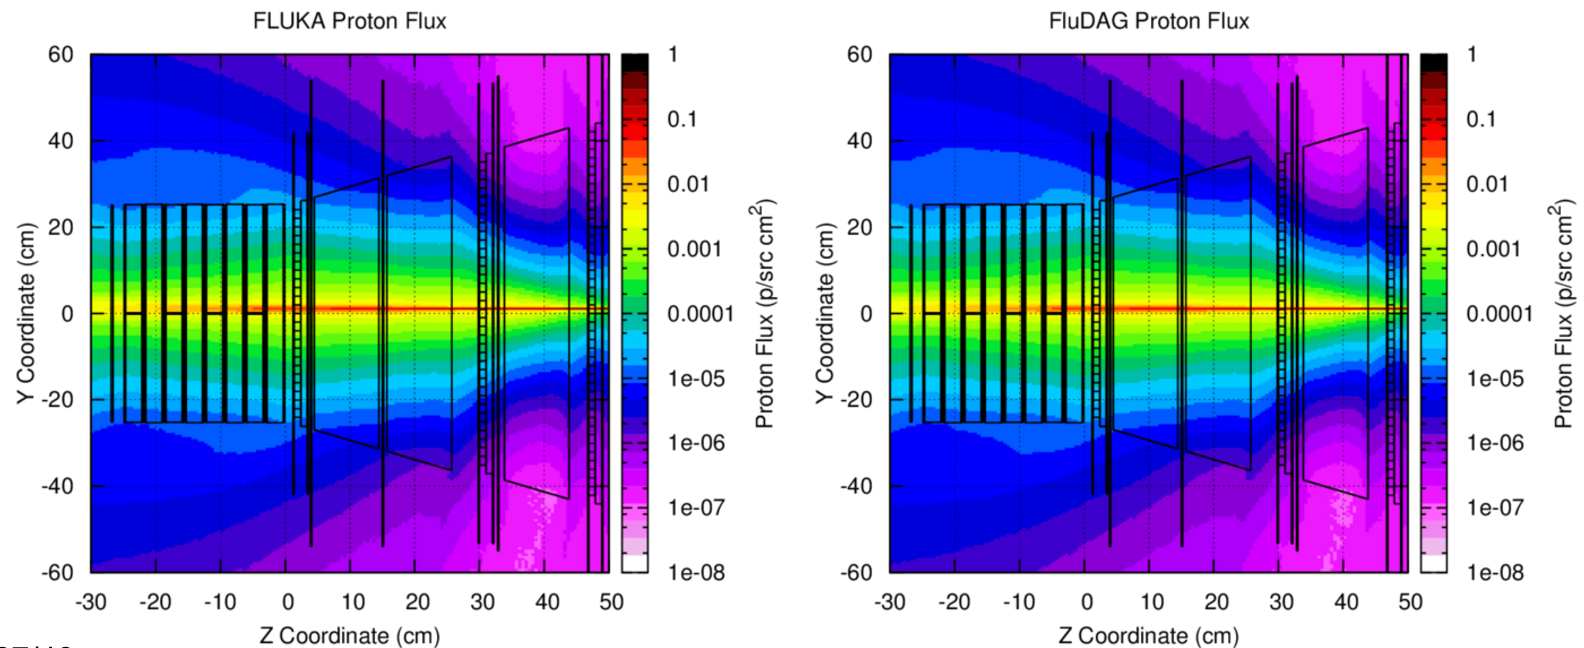
\includegraphics[width=0.7\paperwidth]{../figs/atic_proton_flux.png}
 \caption{Proton flux profile determine in the native FLUKA geometry (left) and the FluDAG geometry (right)}
 \label{fig:atic_proton_flux}
 \end{centering}
\end{figure}
\begin{figure}[ht!]
 \begin{centering}
 \centering
 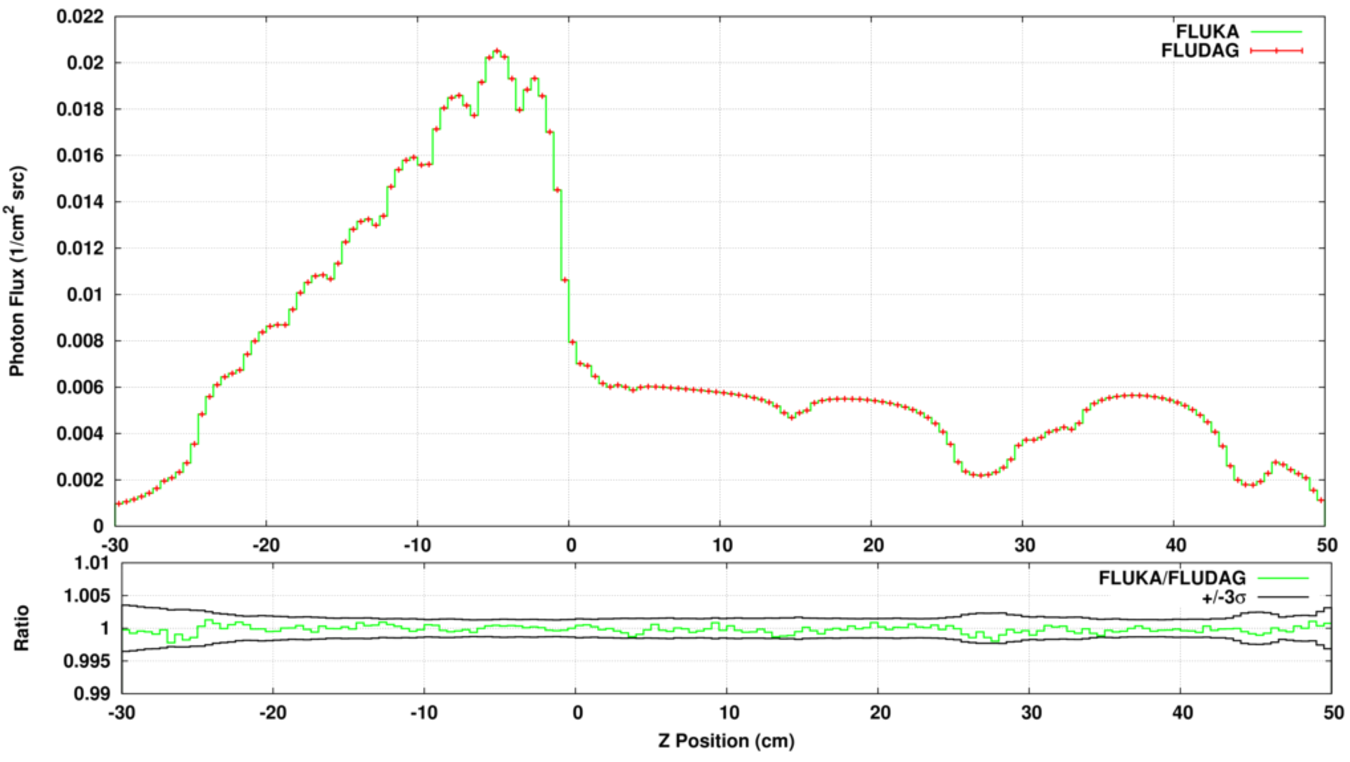
\includegraphics[width=0.7\paperwidth]{../figs/atic_proton_flux_lineout.png}
 \caption{Proton flux profiles, FLUKA as lines, FluDAG as points and the ratio of the profiles (FluDAG/Fluka)}
 \label{fig:atic_proton_flux_lineout}
 \end{centering}
\end{figure}

\begin{figure}[ht!]
 \begin{centering}
 \centering
 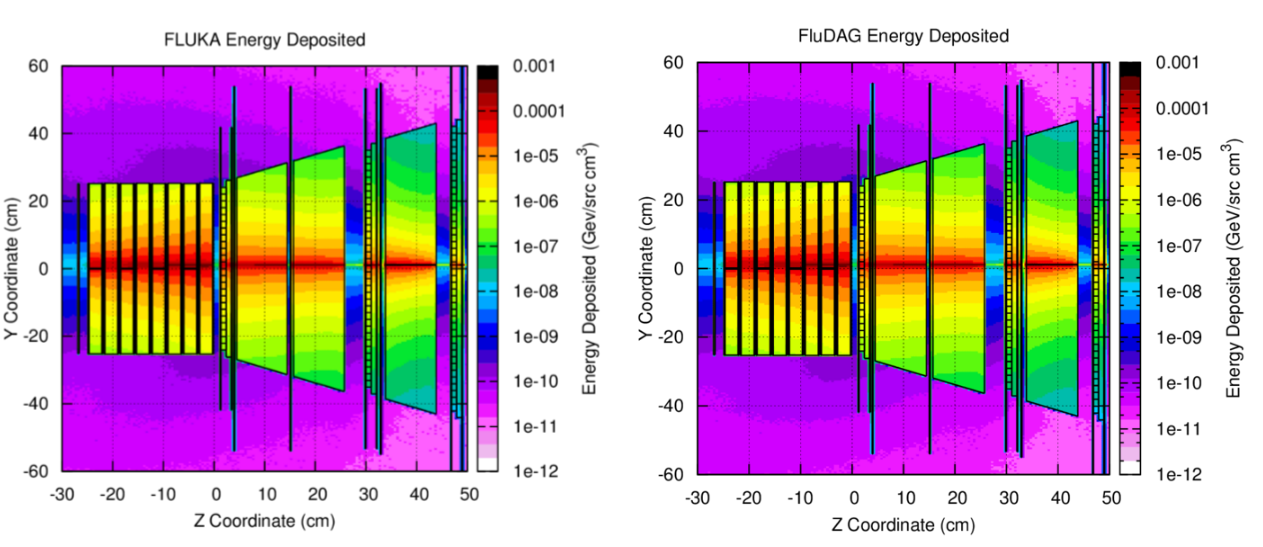
\includegraphics[width=0.7\paperwidth]{../figs/atic_energy_deposition.png}
 \caption{Energy deposition profile determine in the native FLUKA geometry (left) and the FluDAG geometry (right)}
 \label{fig:atic_energy_deposition}
 \end{centering}
\end{figure}
\begin{figure}[ht!]
 \begin{centering}
 \centering
 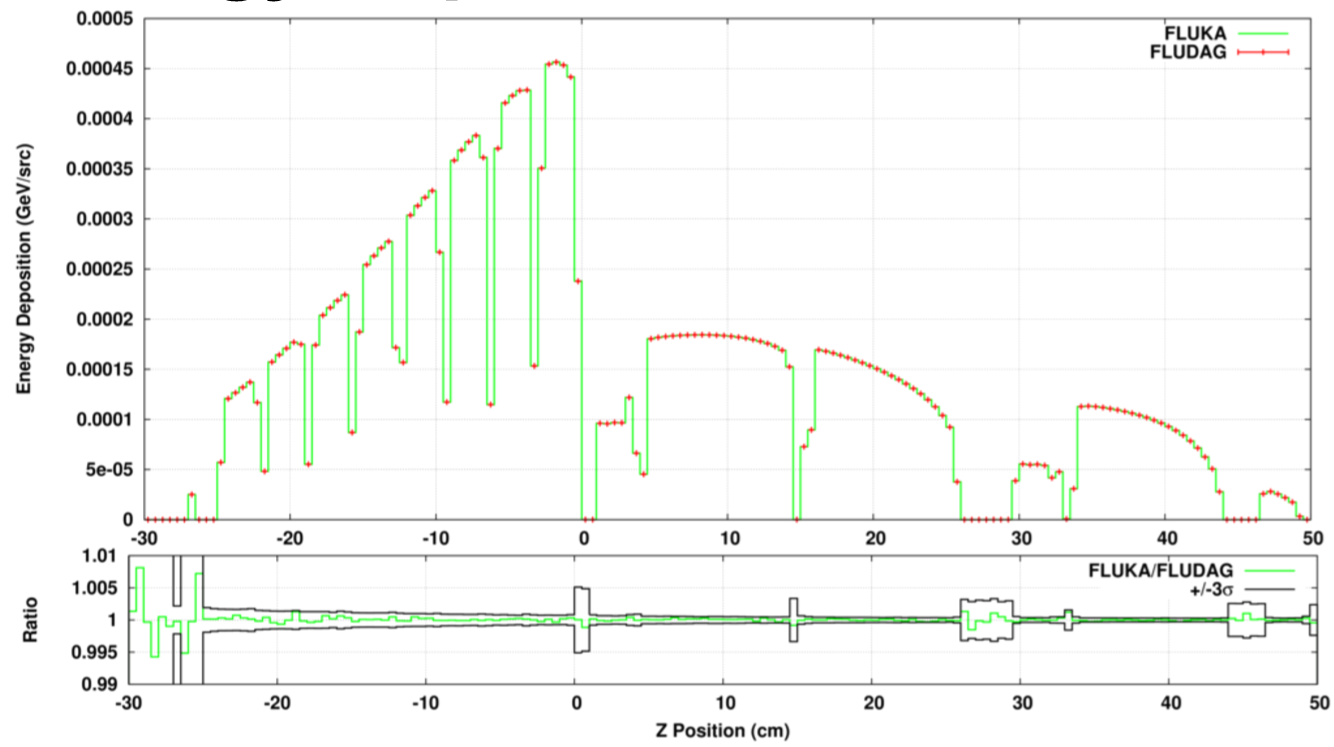
\includegraphics[width=0.7\paperwidth]{../figs/atic_energy_deposition_lineout.png}
 \caption{Energy deposition profiles, FLUKA as lines, FluDAG as points and the ratio of the profiles (FluDAG/Fluka)}
 \label{fig:atic_energy_deposition_lineout}
 \end{centering}
\end{figure}

\begin{figure}[ht!]
 \begin{centering}
 \centering
 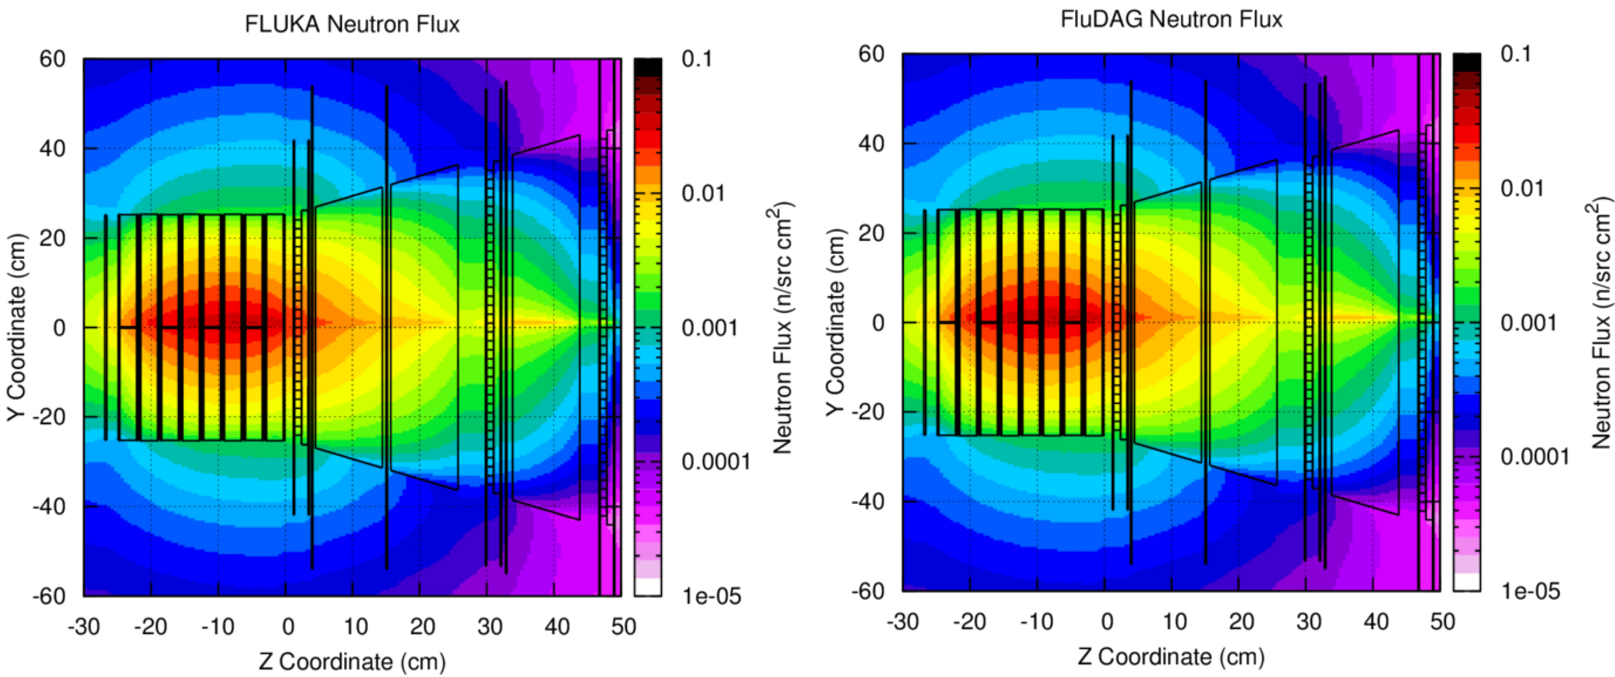
\includegraphics[width=0.7\paperwidth]{../figs/atic_neutron_flux.png}
 \caption{Neutron flux profile determine in the native FLUKA geometry (left) and the FluDAG geometry (right)}
 \label{fig:atic_neutron_flux}
 \end{centering}
\end{figure}
\begin{figure}[ht!]
 \begin{centering}
 \centering
 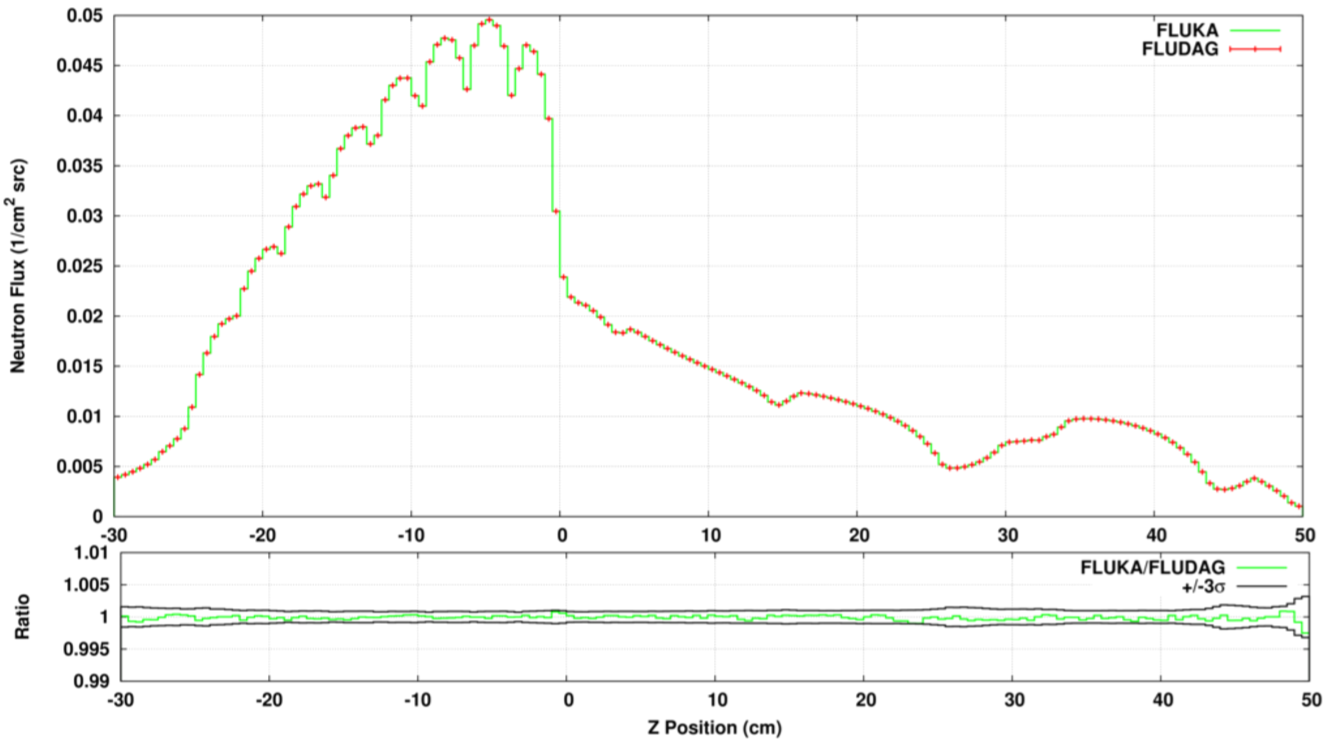
\includegraphics[width=0.7\paperwidth]{../figs/atic_neutron_flux_lineout.png}
 \caption{Neutron flux profiles, FLUKA as lines, FluDAG as points and the ratio of the profiles (FluDAG/Fluka)}
 \label{fig:atic_neutron_flux_lineout}
 \end{centering}
\end{figure}

\begin{figure}[ht!]
 \begin{centering}
 \centering
 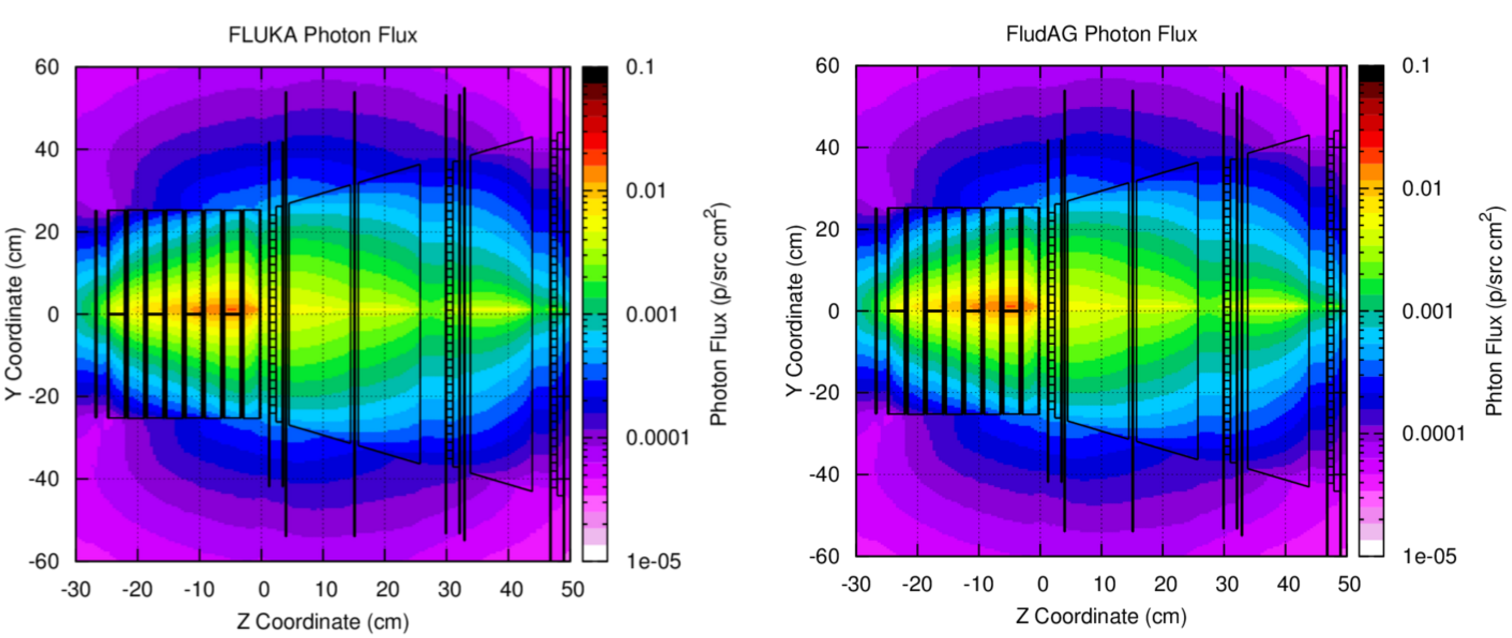
\includegraphics[width=0.7\paperwidth]{../figs/atic_photon_flux.png}
 \caption{Photon flux profile determine in the native FLUKA geometry (left) and the FluDAG geometry (right)}
 \label{fig:atic_photon_flux}
 \end{centering}
\end{figure}
\begin{figure}[ht!]
 \begin{centering}
 \centering
 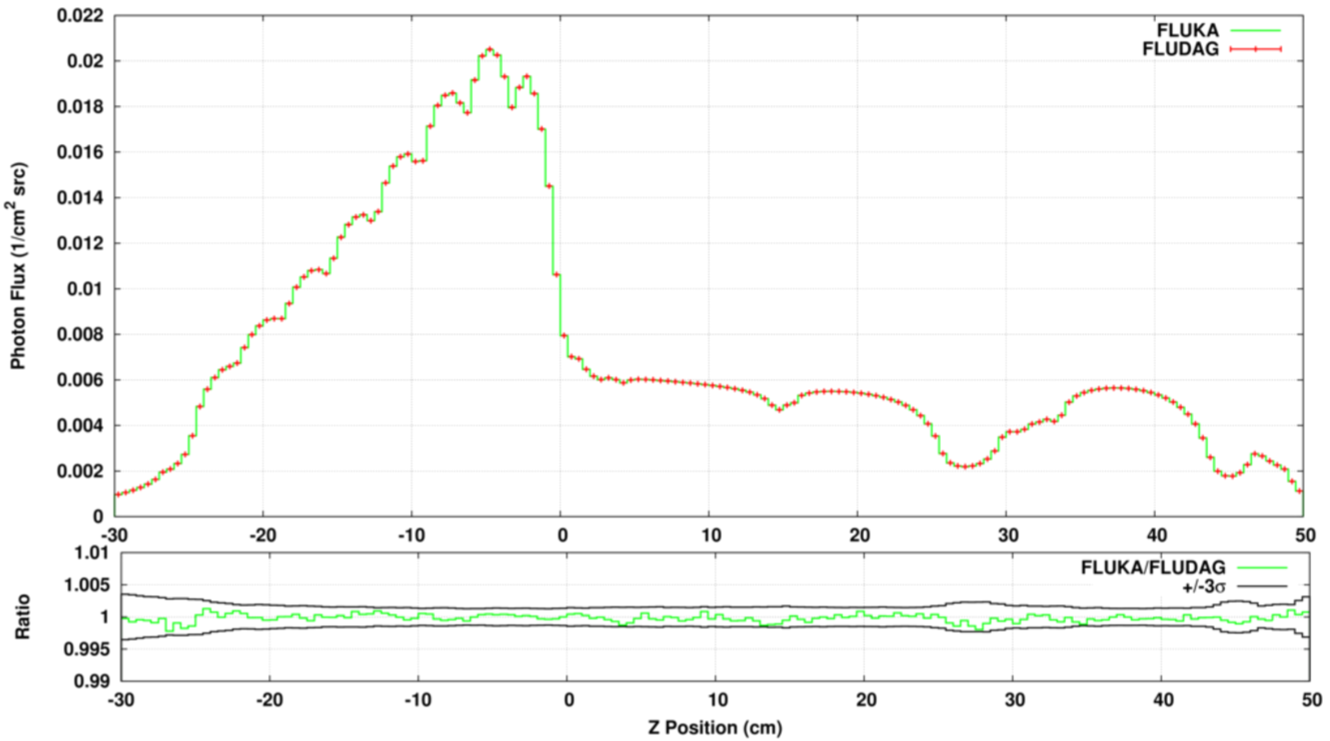
\includegraphics[width=0.7\paperwidth]{../figs/atic_photon_flux_lineout.png}
 \caption{Photon flux profiles, FLUKA as lines, FluDAG as points and the ratio of the profiles (FluDAG/Fluka)}
 \label{fig:atic_photon_flux_lineout}
 \end{centering}
\end{figure}

\clearpage
\subsubsection{AlAuAl}
The AlAuAl (aluminium-gold-aluminium) benchmark originated from the development of FLUGG. The benchmark is 
specifically designed to stress electron transport in very thin layers. The geometry of the setup is shown in
Figure \ref{fig:alaual_fig}.

\begin{figure}[ht!]
 \begin{centering}
 \centering
 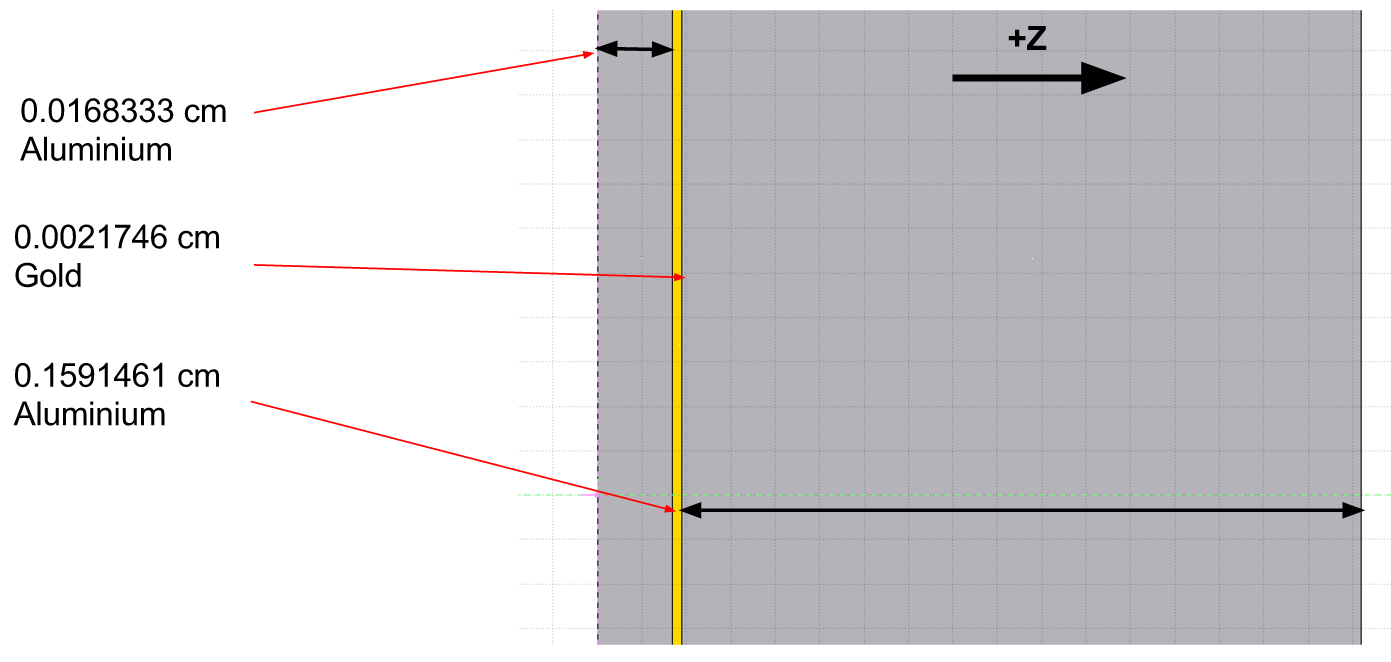
\includegraphics[width=0.7\paperwidth]{../figs/alaual_geom.png}
 \caption{The geometry of the setup for the AlAuAl benchmark (FLUKA geometry shown)}
 \label{fig:alaual_fig}
 \end{centering}
\end{figure}

The source is a 1 MeV pencil electron beam pointed in the postive z direction, with particles starting at 0,0, -10.0 cm. The CAD model
for the FluDAG was created by exporting the native FLUKA geometry to MCNP format, then using mcnp2cad [ref] the CAD model was created. 
Each calculation was run with 5.0$\times$10$^5$ with 20 batches.

\begin{figure}[ht!]
 \begin{centering}
 \centering
 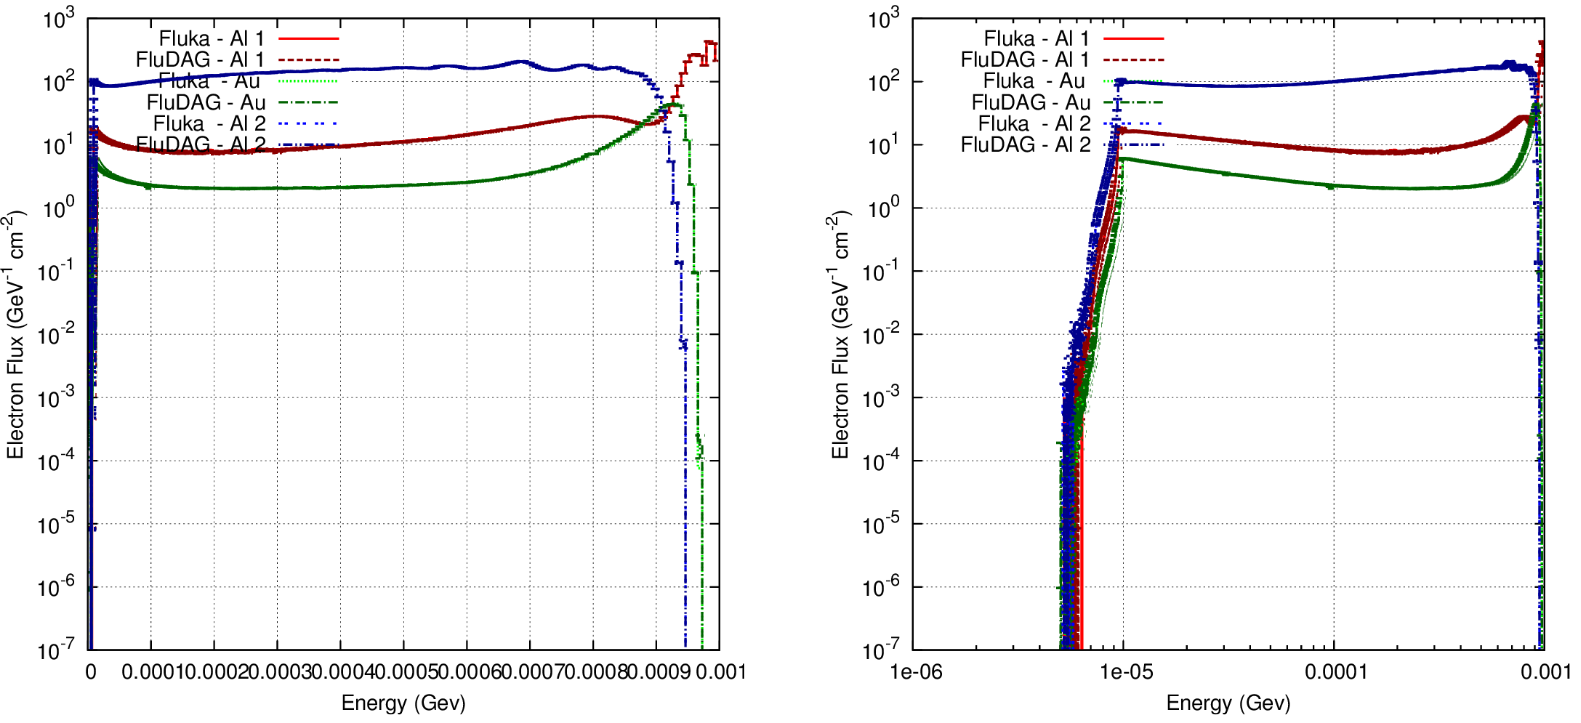
\includegraphics[width=0.7\paperwidth]{../figs/alaual_spectra_lin_log.png}
 \caption{}
 \label{fig:alaual_spectra_linlog}
 \end{centering}
\end{figure}

\begin{figure}[ht!]
 \begin{centering}
 \centering
 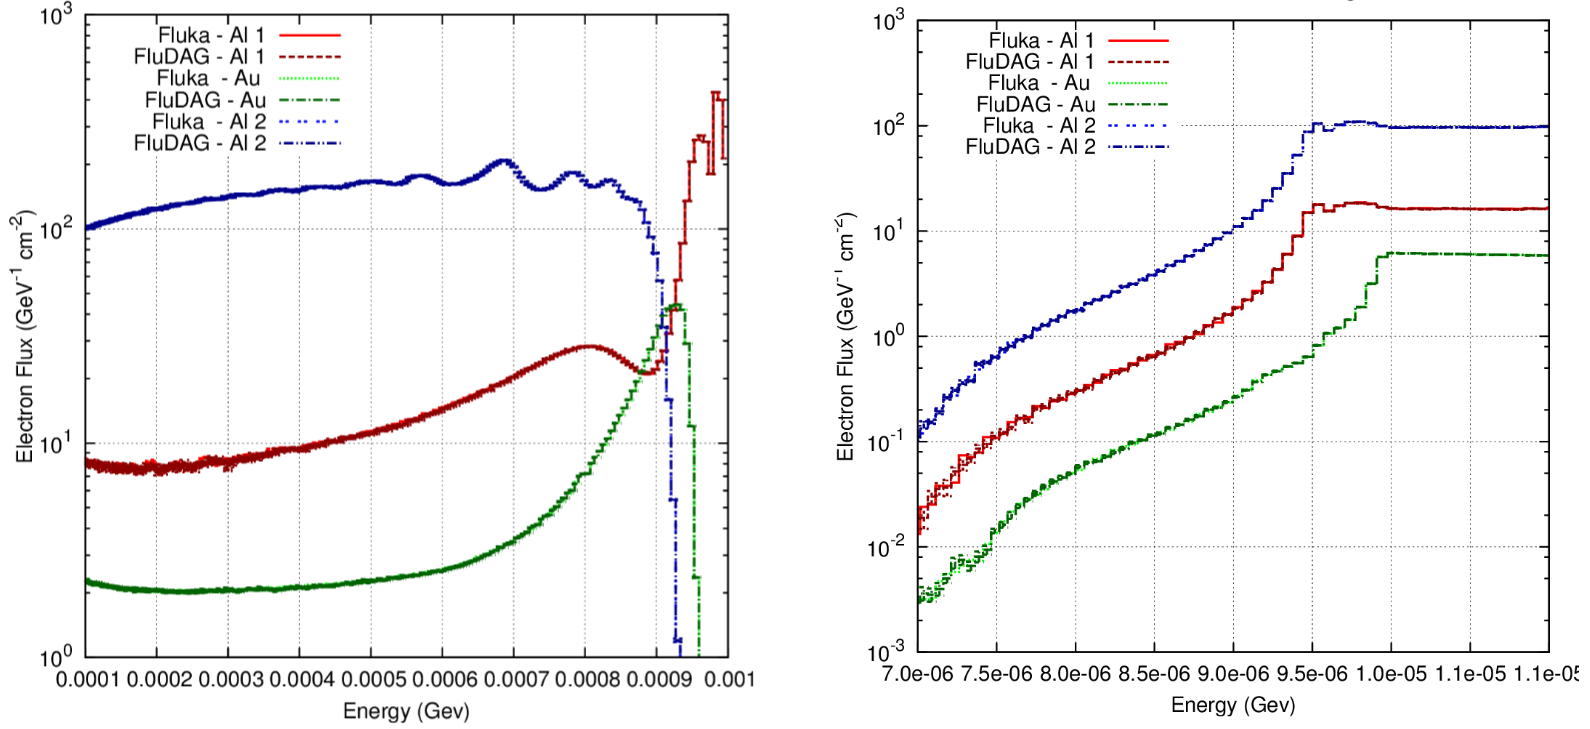
\includegraphics[width=0.7\paperwidth]{../figs/alaual_spectra_log_log.png}
 \caption{}
 \label{fig:alaual_spectra_loglog}
 \end{centering}
\end{figure}

The suite of results displayed were shown to the FLUKA team at CERN during the FLUKA collaboration meeting
in 2015, it was agreed then that the co-oberation between the the results are excellent and show no artifacts
in the transport of electrons. 

\clearpage
\subsubsection{Magnetic Field \& Spheres}
During the devlopment of FLUGG a specific test case gave particularly pathogenic behaviour for electrons crossing
boundaries between cells, the test is subsequently known as MagnSph and the geometry is shown in Figure 
\ref{fig:magnsph_geom}. This test is particularly pathogenic for electron transport due to some of the peculiarities
of electron transport in general and some of the FLUKA specific steps for electrons that are different than other 
particles. The true geometry is composed of cylinders and spheres which numerically touch. 
\\
\\
It is not possible to represent the true geometry of this benchmark in CAD since it is not possible to resolve
numerically touching, specifically with the Cubit based workflow, ACIS can only distinguish vertices as being
distinct entities when they are greater than 1e-6 cm apart. In this instance we found that the problem as originally
defined resulted in several imprint and merge issues. Reducing the radii of cylinder from 0.5 to 0.49999 and the radii
of the spheres from 0.3 to 0.29999 resulted in no issues regarding imprinting or merging. However, changing the radii
to 0.499999 and 0.299999 respecively had the same issues as the unmodified model. Thus, the final model used for the
benchmark calculations were has radii of cylinders and spheres of 0.49999 and 0.29999 respectively.  

\begin{figure}[ht!]
 \begin{centering}
 \centering
 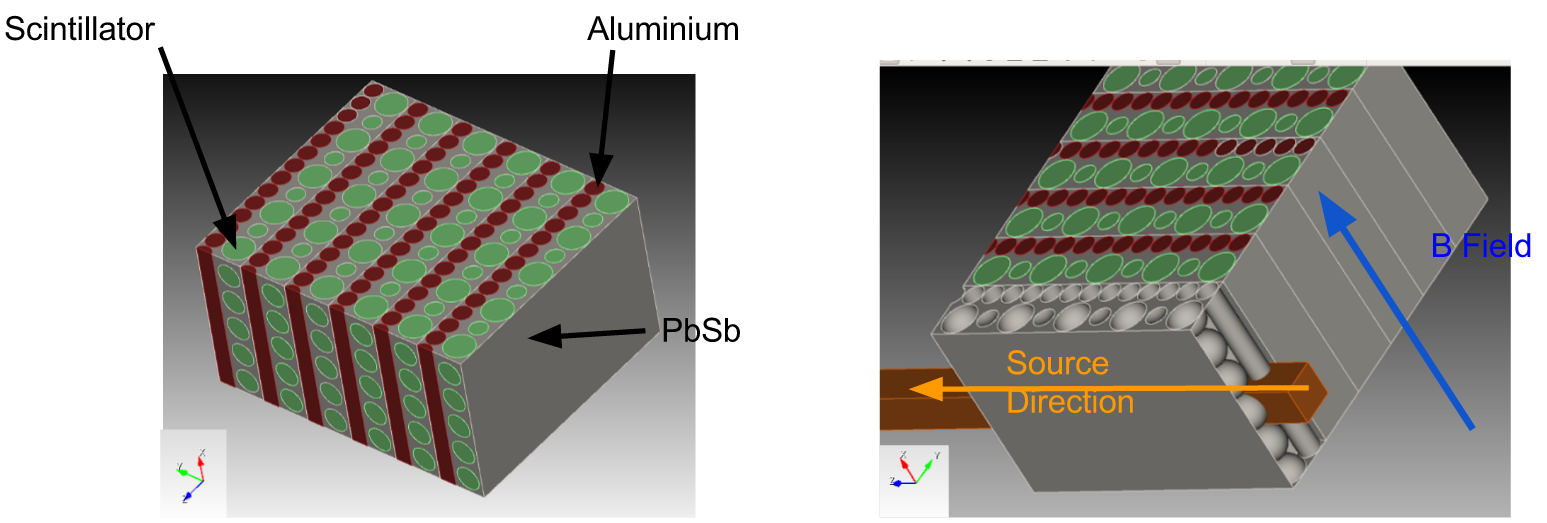
\includegraphics[width=0.7\paperwidth]{../figs/magnsph_geom.png}
 \caption{}
 \label{fig:magnsph_geom}
 \end{centering}
\end{figure}

The source is a square cross sectioned beam of side 1 cm containing positrons at 1 GeV, starting at 2,4,-1 cm directed into the postive
z direction. There is a uniform magnetic field of 60 T directed along the x direction. 

\begin{figure}[ht!]
 \begin{centering}
 \centering
 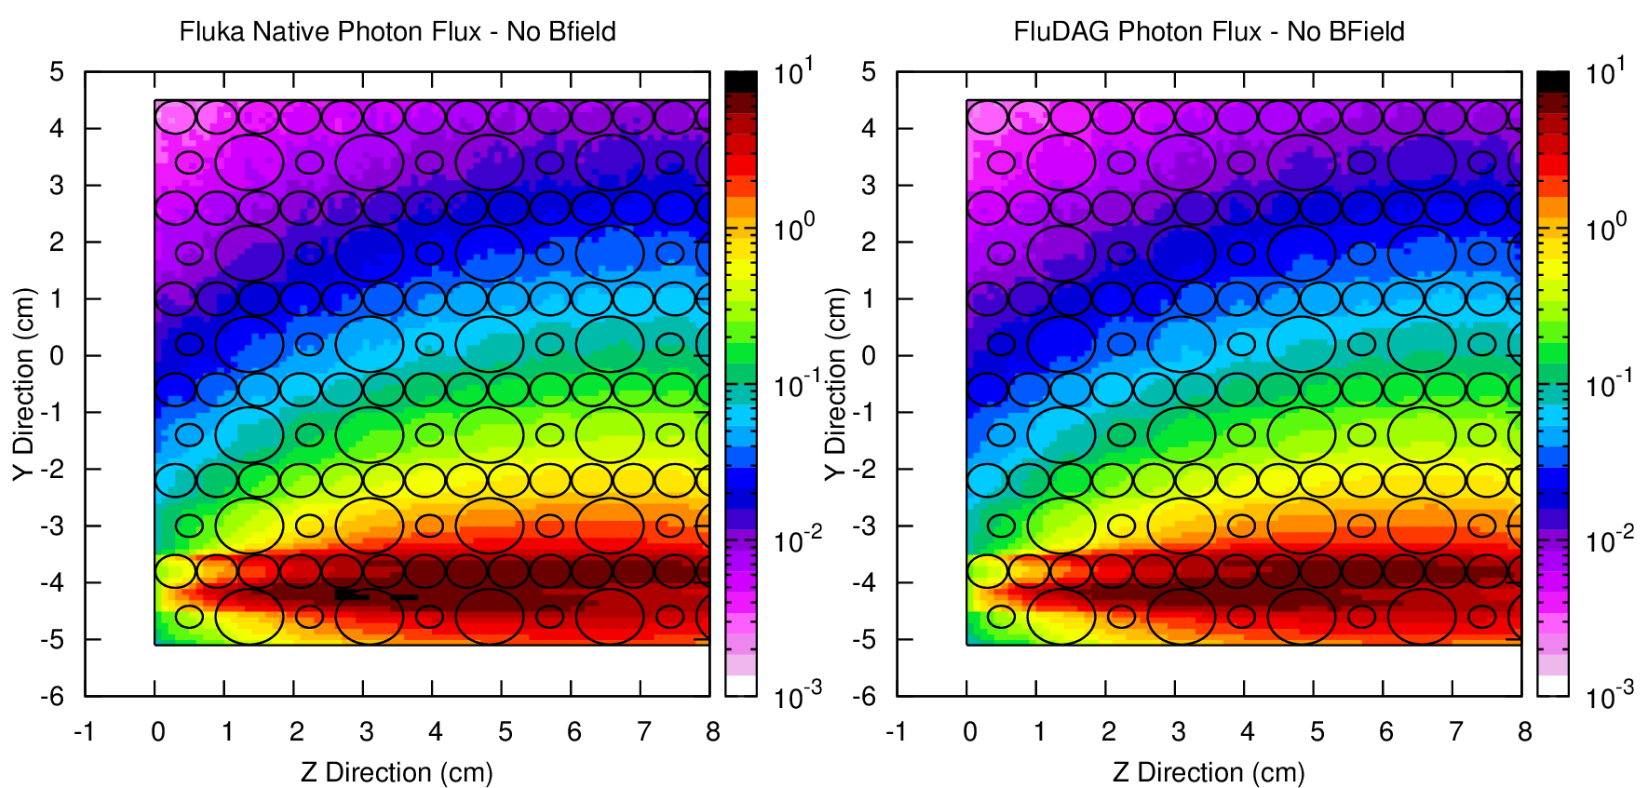
\includegraphics[width=0.9\paperwidth,angle=90]{../figs/magnsph_photon_nob.png}
 \caption{}
 \label{fig:magnsph_photon_nob}
 \end{centering}
\end{figure}

\begin{figure}[ht!]
 \begin{centering}
 \centering
 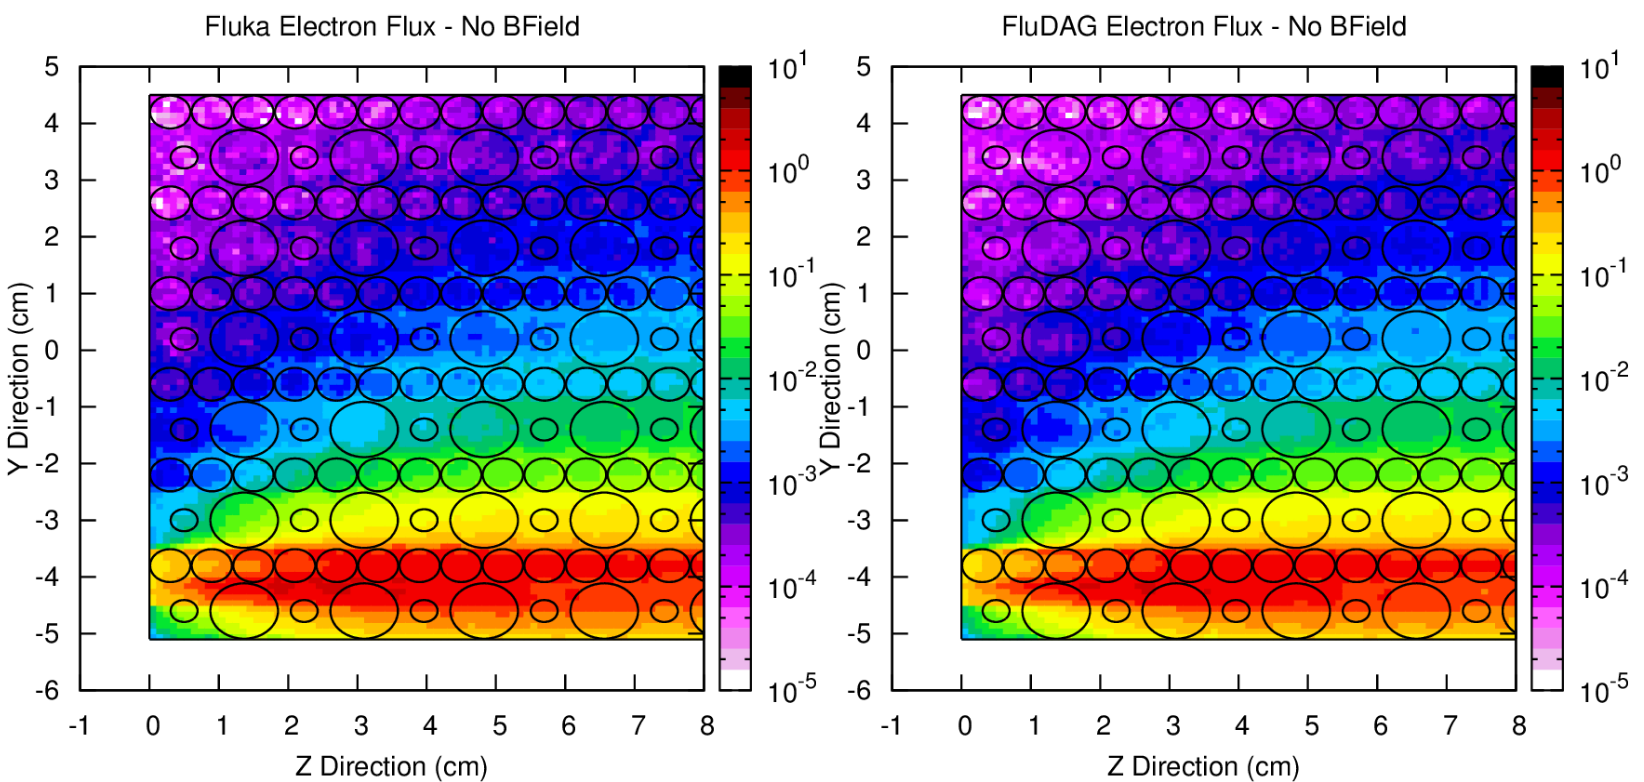
\includegraphics[width=0.9\paperwidth,angle=90]{../figs/magnsph_electron_nob.png}
 \caption{}
 \label{fig:magnsph_electron_nob}
 \end{centering}
\end{figure}

\begin{figure}[ht!]
 \begin{centering}
 \centering
 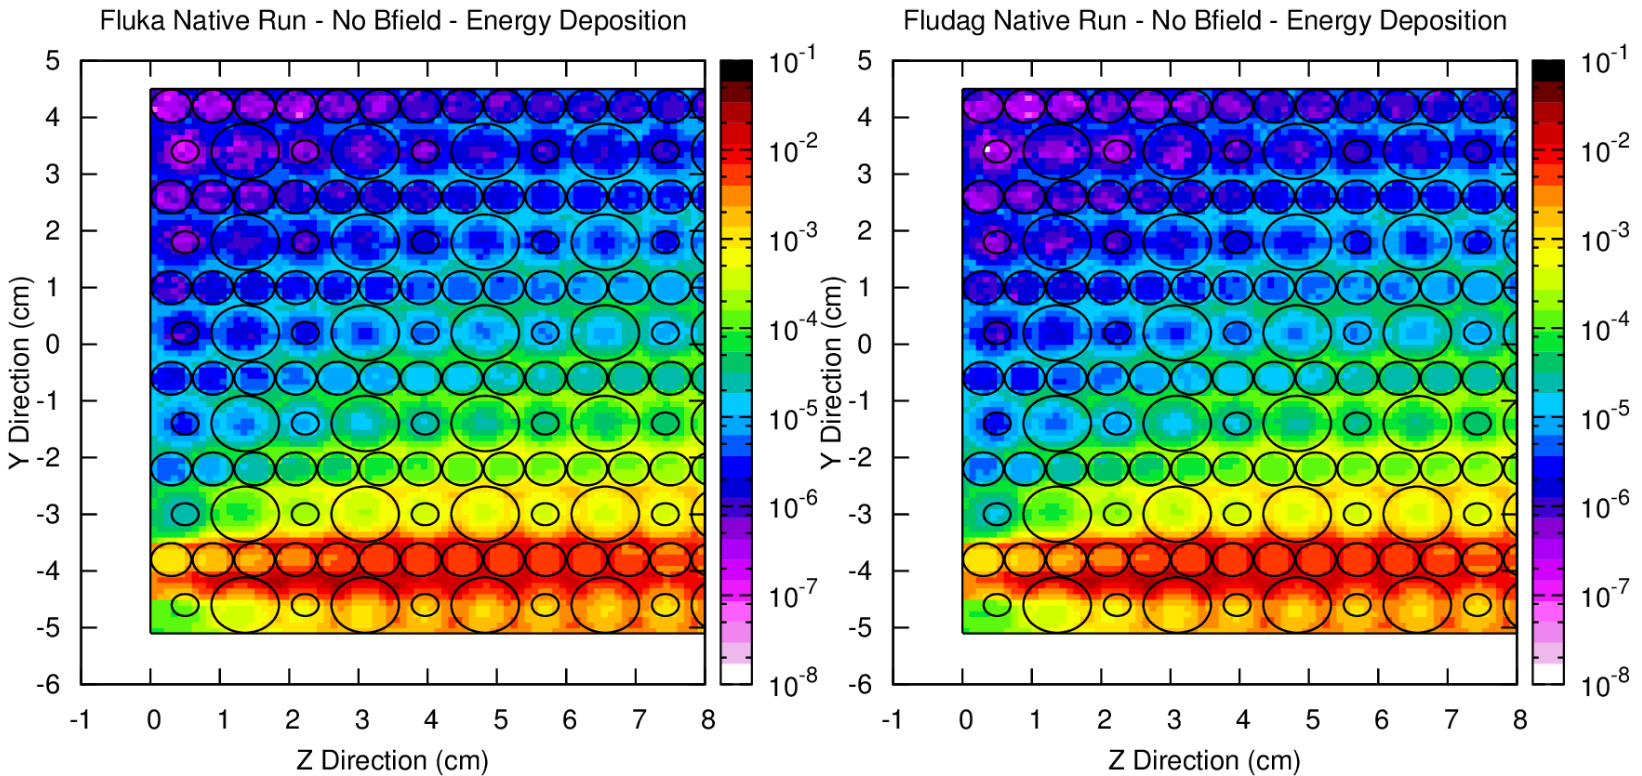
\includegraphics[width=0.9\paperwidth,angle=90]{../figs/magnsph_energy_nob.png}
 \caption{}
 \label{fig:magnsph_energy_nob}
 \end{centering}
\end{figure}

\begin{figure}[ht!]
 \begin{centering}
 \centering
 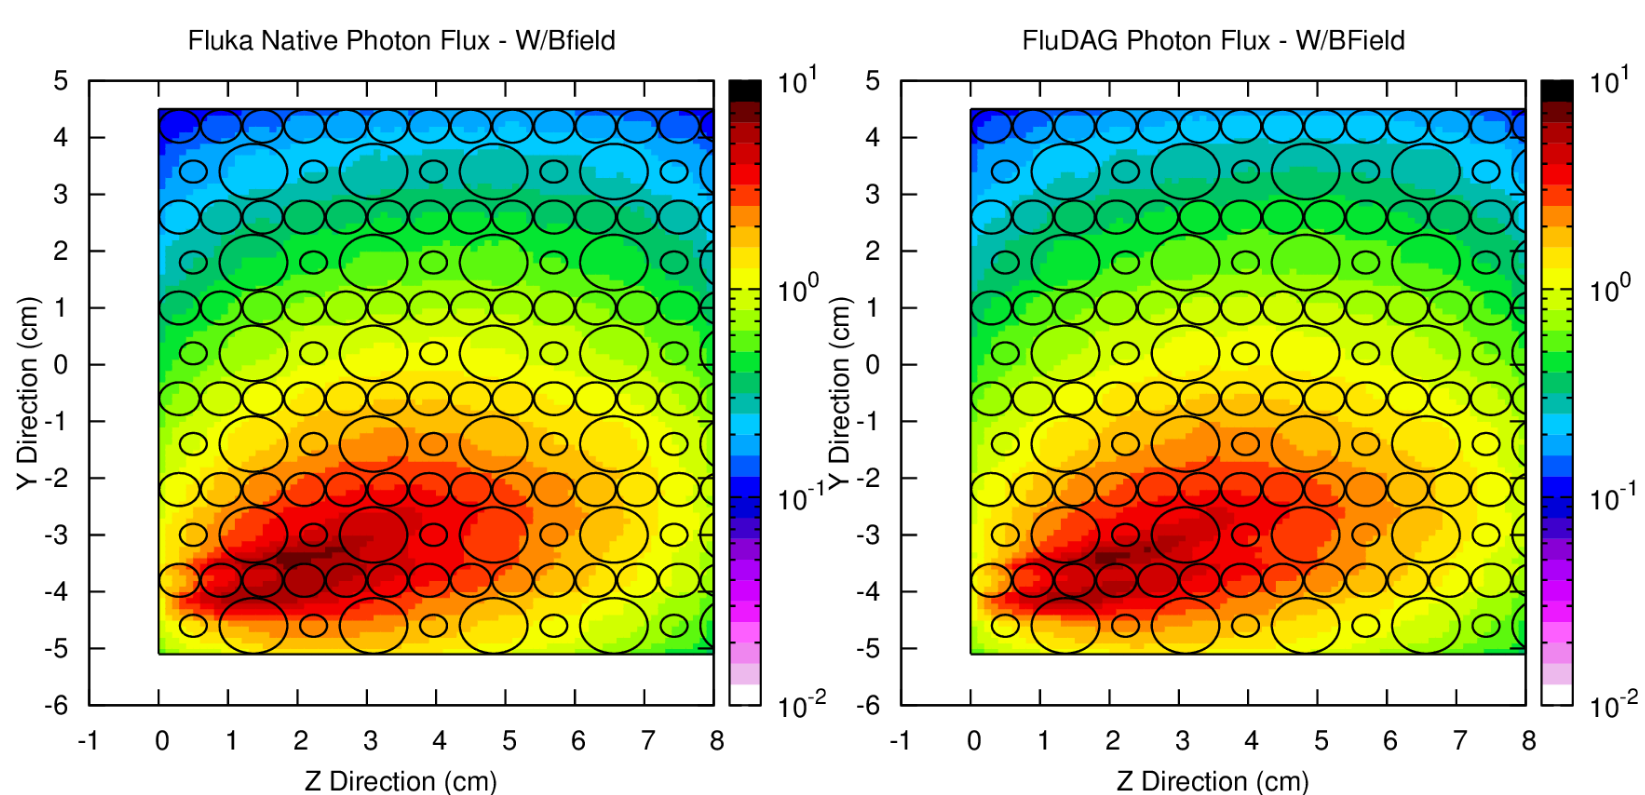
\includegraphics[width=0.9\paperwidth,angle=90]{../figs/magnsph_photon_b.png}
 \caption{}
 \label{fig:magnsph_photon_b}
 \end{centering}
\end{figure}

\begin{figure}[ht!]
 \begin{centering}
 \centering
 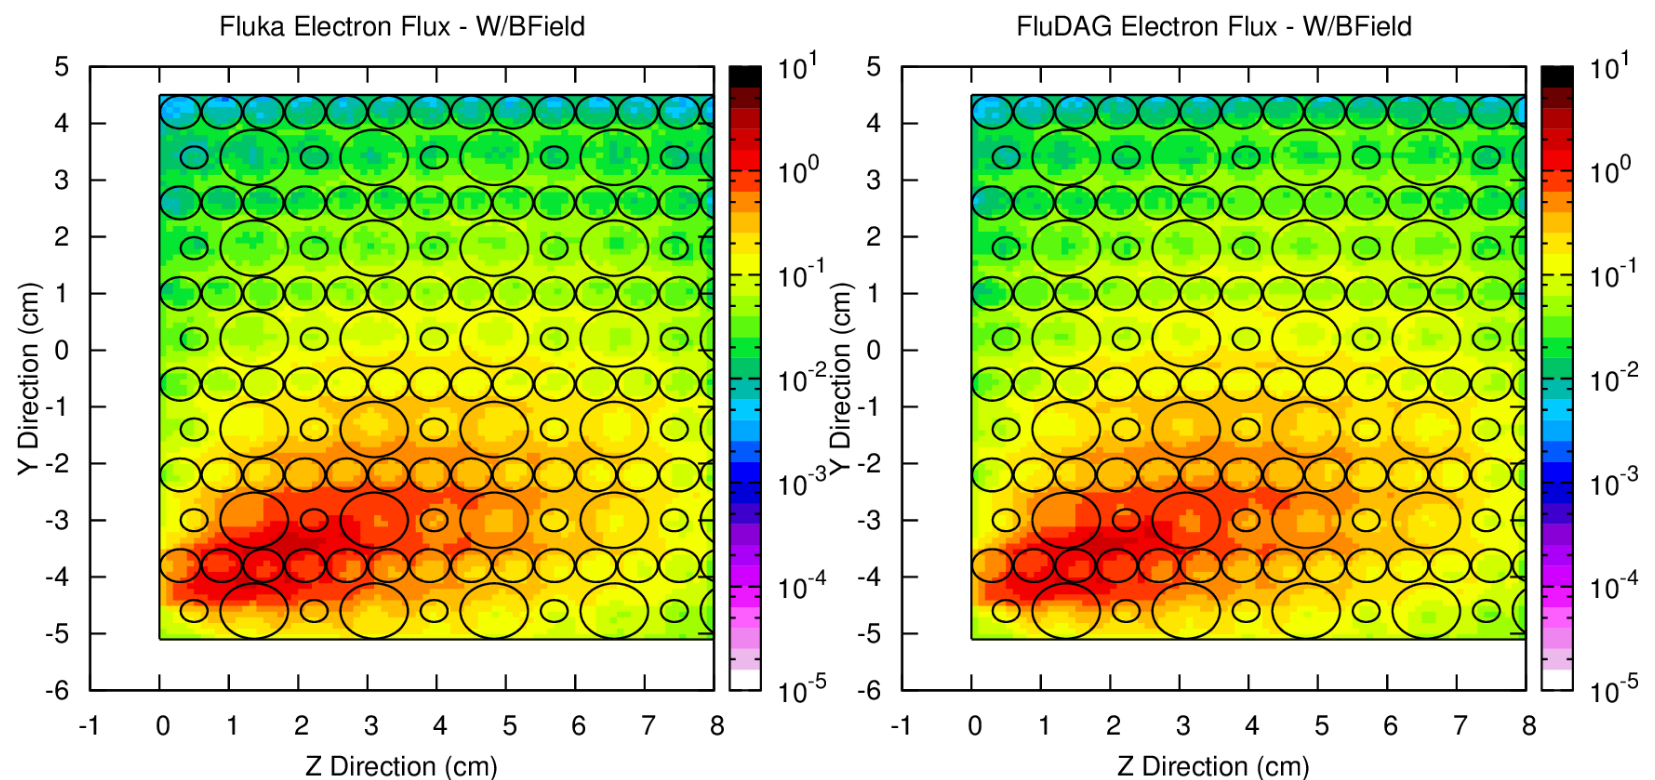
\includegraphics[width=0.9\paperwidth,angle=90]{../figs/magnsph_electron_b.png}
 \caption{}
 \label{fig:magnsph_electron_b}
 \end{centering}
\end{figure}

\begin{figure}[ht!]
 \begin{centering}
 \centering
 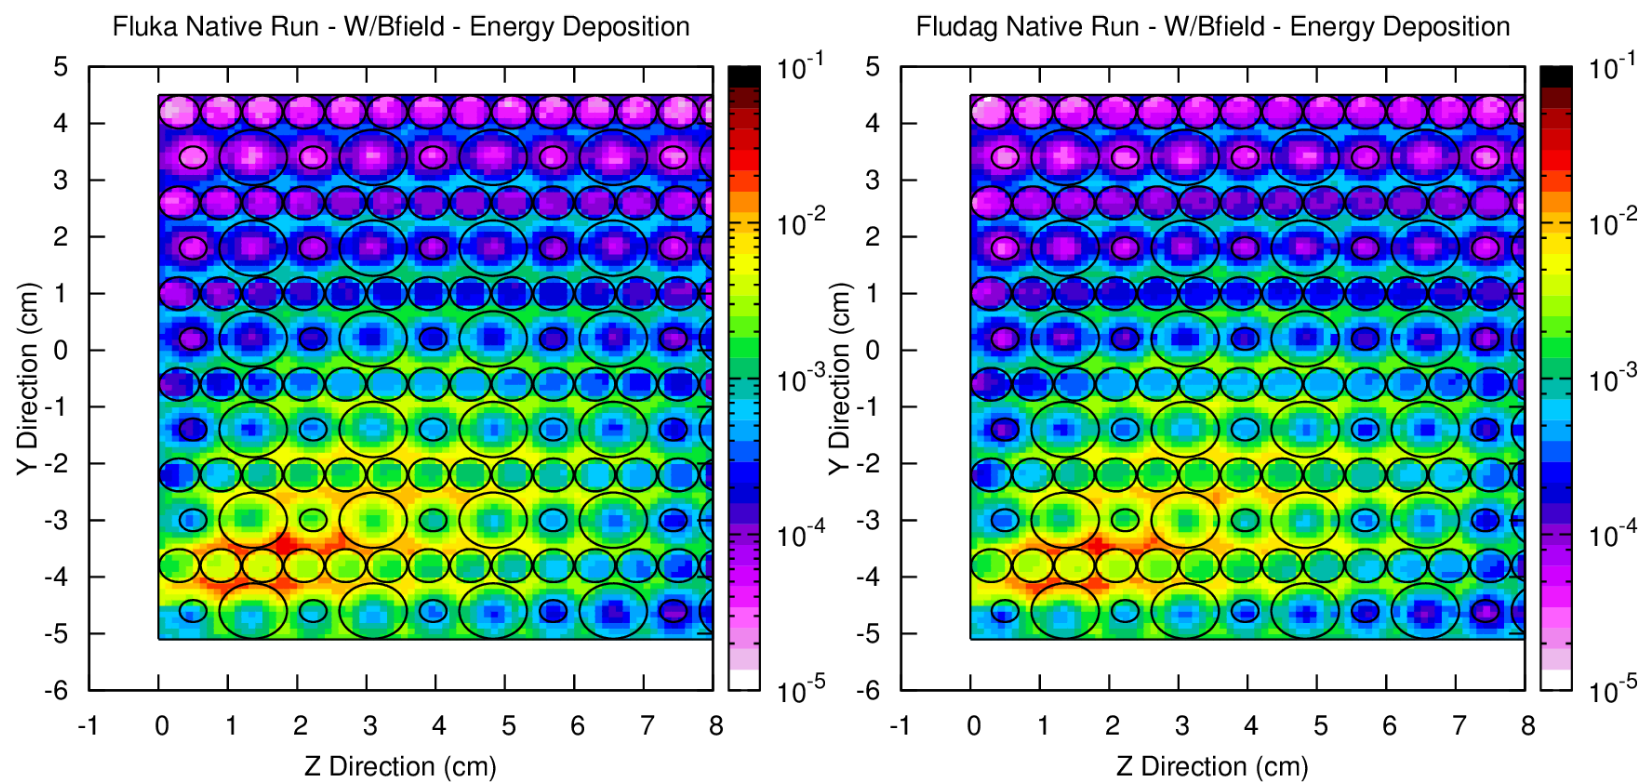
\includegraphics[width=0.9\paperwidth,angle=90]{../figs/magnsph_energy_b.png}
 \caption{}
 \label{fig:magnsph_energy_b}
 \end{centering}
\end{figure}


